%!TEX root = ../main.tex

\section{Attacks on bitcoin mining}
\label{sec:attack}
In Section~\ref{sec:fork} we have shown that continued forks are
extremely unlikely, if nodes stick to the longest chain rule and
do not disturb the network latency.

In the following we first look at two ways to deviate from the 
longest chain rule, stubborn mining and selfish (hidden) mining.
And we look at network attacks that might be performed.

We first look at those attacks from the perspective of fair mining.
Then we look at them from the perspective of a double spend.

\begin{definition}
Mining, or block creation is \emph{fair} if a node that possesses $\alpha$ 
percent of the hashing power in the network ends up publishing $\alpha$
blocks in the longest chain.
\end{definition}


\subsection{Stubborn mining}
A node does perform stubborn mining, if it does not abandon the 
current chain for the longest chain. Thus it does not follow the longest chain rule.

More precisely, if there exist two blockchains $c_1$ and $c_2$ 
and $c_2$ contains one more block than $c_1$. Thus the initial state is as shown in Figure~\ref{fig:fork}.
A stubborn node that has published a block in $c_1$ that is not
part of $c_2$ will continue to try and extend $c_1$ until either
$c_1$ becomes the longest. We assume that if the difference between
$c_1$ and $c_2$ increases, the stubborn node will abandon $c_1$.

\begin{theorem}
	
	Stubborn mining does not increases the expected outcome of a node, if
	the node controls less than $\alpha=0.42$ of the hashing power in the network.
	
\end{theorem}
\begin{proof}
	We model this system as a markov chain with 4 states.
	\begin{itemize}
		\item[Loose] where chain $c_1$ was extended faster than $c_2$.
		\item[$-1$] where chain $c_1$ is one block longer than chain $c_2$.
		\item[$0$] where $c_1$ and $c_2$ are equally long.
		\item[Win] where chain $c_2$ became the longest chain.
	\end{itemize}
	
	We ignore the probability that additional forks occur on $c_2$ but 
	note that they would increase the profitability of stubborn mining.
	Assume the probability that the attacker finds a block is $\alpha$,
	while $\beta=1-\alpha$ is the probability that the remaining miners find a block. The states and the transition probabilities are shown in Figure~\ref{fig:stubborn}.
	\begin{figure}
	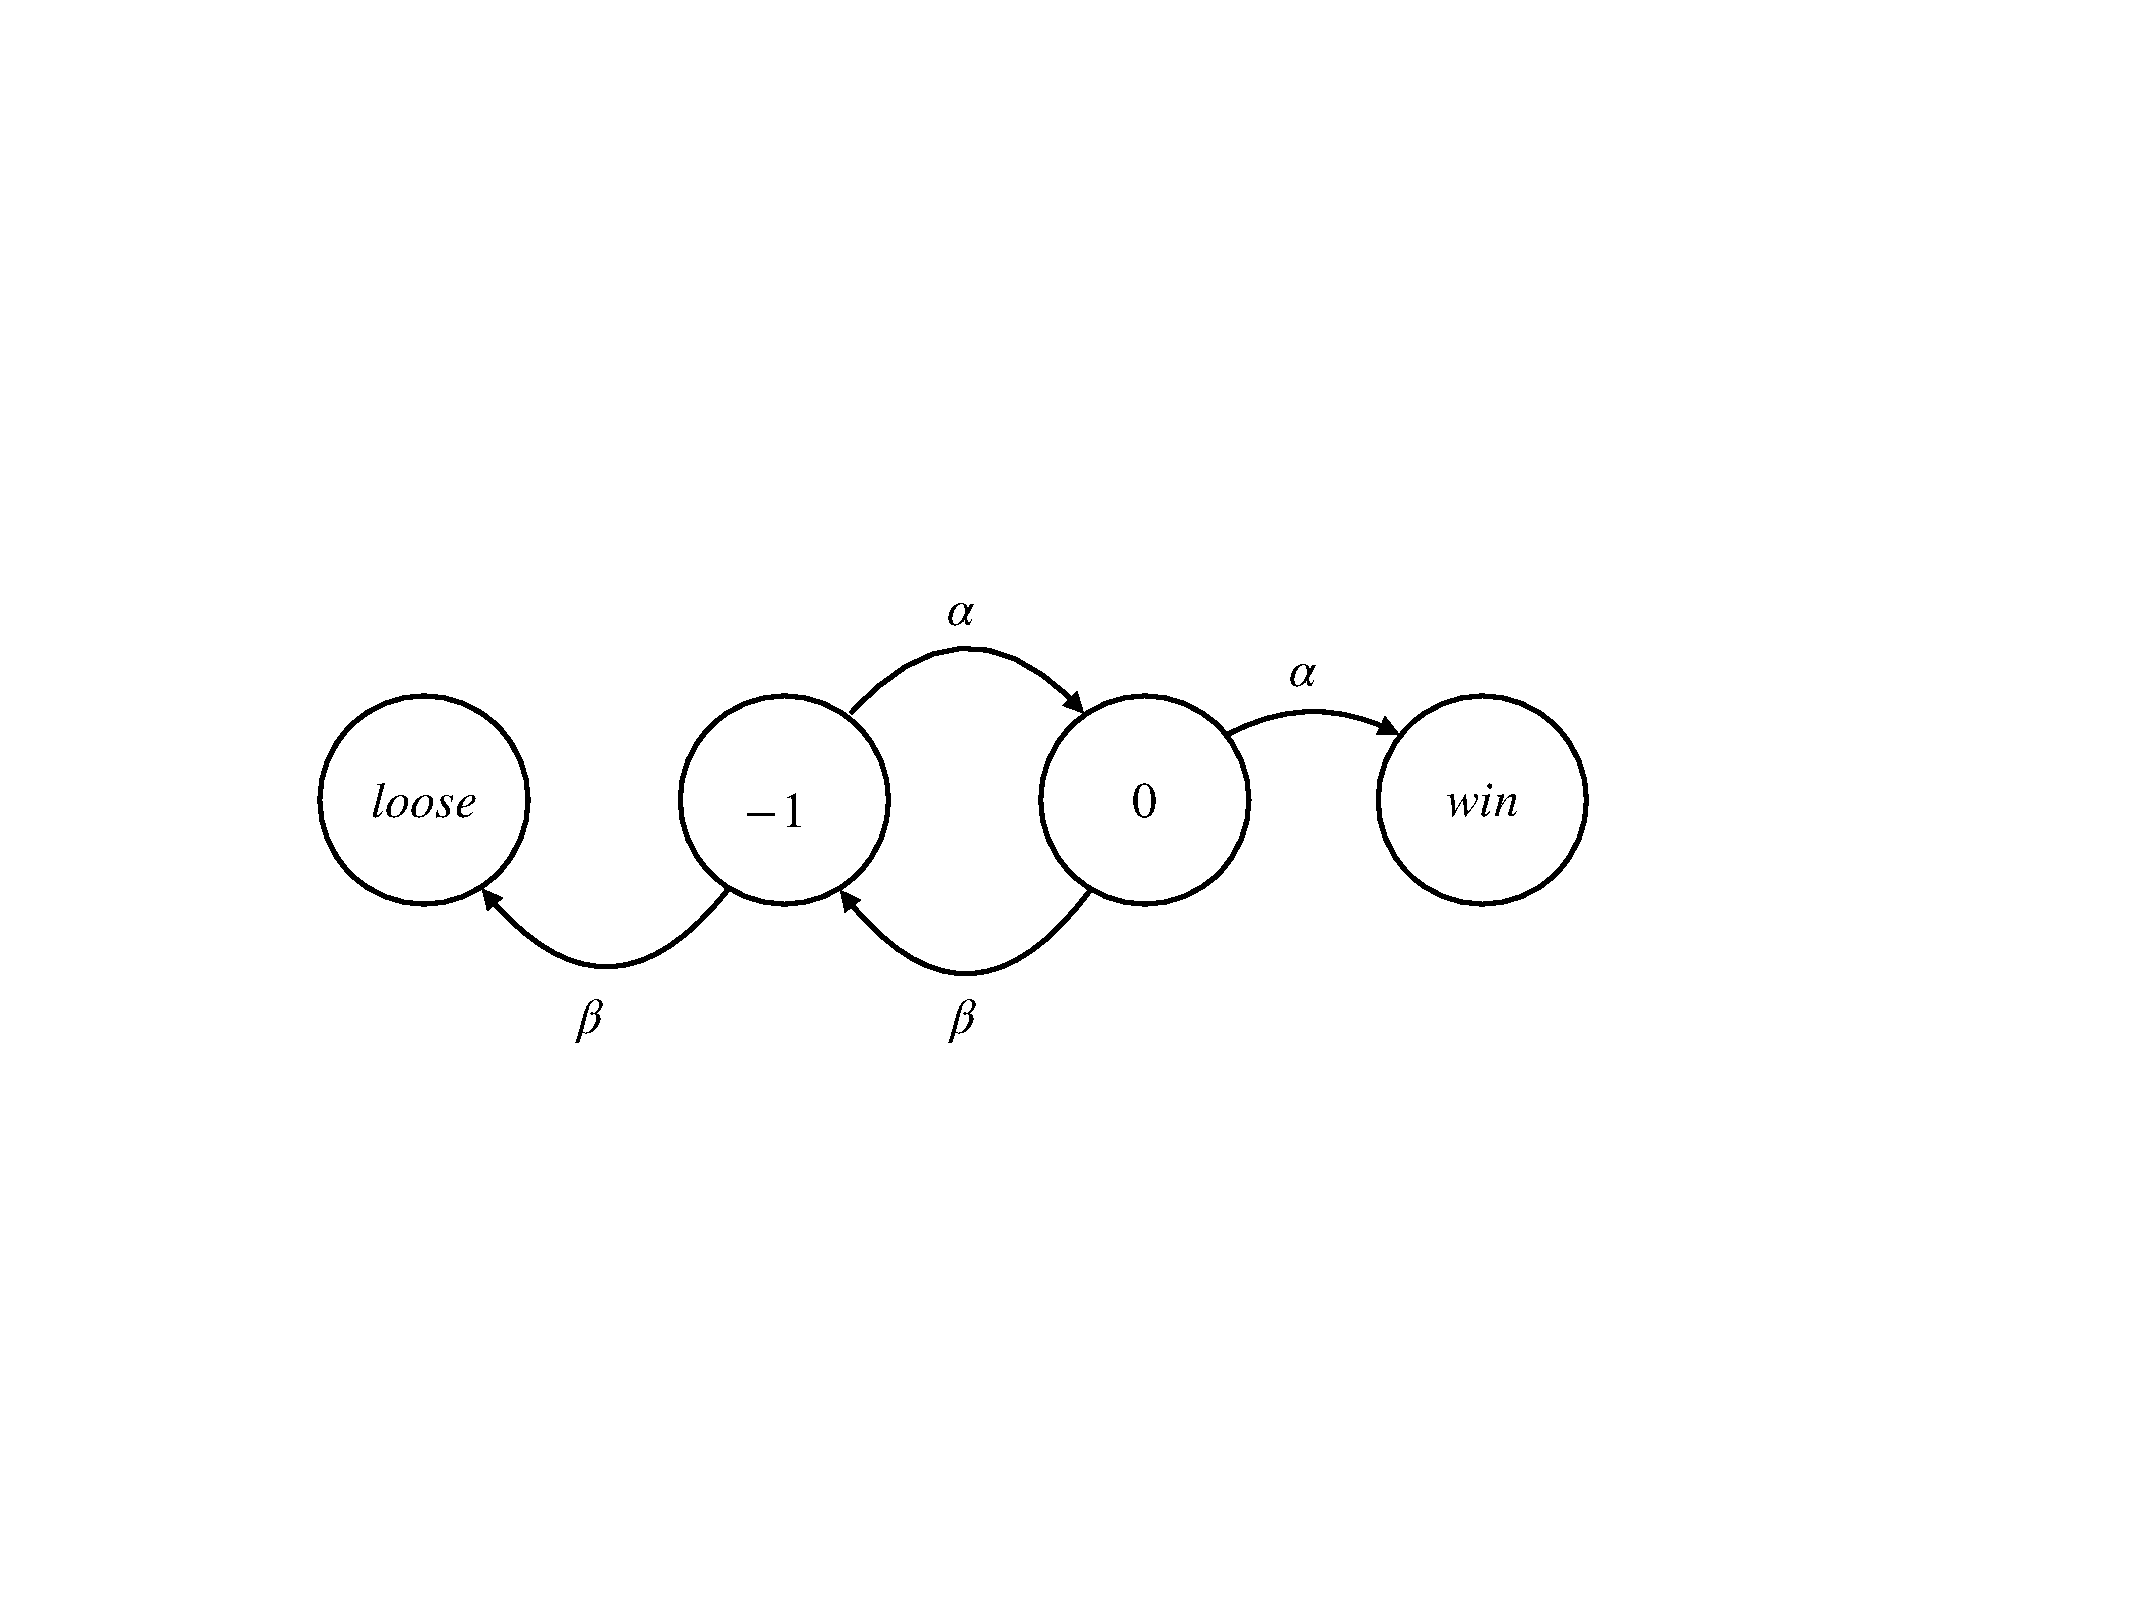
\includegraphics[width=\textwidth]{fig/StubbornMining}
	\caption{Stubborn mining states and transitions.}
	\label{fig:stubborn}
	\end{figure}
	
	We now calculate the expected number of blocks the Attacker receives with and without doing the attack. 
	For the attack we consider the following cases:
	\begin{itemize}
		\item With probability $\beta$ the attacker loses in the first step and receives no blocks.
		\item With probability $\alpha\cdot \alpha$ the attacker mines two blocks. He receive 3 blocks in total.
		\item With probability $\alpha\cdot\beta\cdot \alpha\cdot \alpha$ the process goes through states $-1\mapsto 0 \mapsto -1 \mapsto 0 \mapsto win$.
		In this case the attacker gets 4 blocks.
	\end{itemize}
	Extending the above cases, and omitting those that give 0 blocks,
	$E_{Attack}$ the expected number of blocks is:
	\begin{align}
		E_{Attack}&=\sum_{i=0}(i+3)\alpha^{i+2}\beta^{i}\\
				  &=3\alpha^2+\alpha\beta\left(\sum_i=0(i+3)\alpha^{i+2}\beta^i +\sum_{i=0}\alpha^{i+2}\beta^i\right)\\
				  &=3\alpha^2+\alpha\beta\left(E_{Attack} +\frac{\alpha^2}{1-\alpha\beta}\right)
	\end{align}
	In step (3.2) we used the formula for a geometric sum.
	Solving the above for $E_{Attack}$ gives
	\[
		E_{Attack}=(3+\alpha\beta)\frac{\alpha^2}{1-\alpha\beta}
	\]
	
	To compute the average number of blocks, the attacker would receive if it did not follow the attack, we note that the he gets one block every time an edge with probability $\alpha$ is traversed. We get the following cases.
	\begin{itemize}
		\item With probability $\alpha\cdot \alpha$ the node mines two blocks.
		\item With probability $\alpha\cdot\beta\cdot \beta$ the process goes through states $-1\mapsto 0 \mapsto -1 \mapsto loose$. The node mines 1 block.
		\item With probability $\alpha\cdot\beta\cdot \alpha\cdot \alpha$ the process goes through states $-1\mapsto 0 \mapsto -1 \mapsto 0 \mapsto win$.
		In this case the node gets 3 blocks.
	\end{itemize}
	Continuing the above analysis, we see that the average number of blocks received when not following the above state machine, but not following the attack, is:
	\[
	E_{NoAttack}=\sum_{i=0}(i+2)\alpha^{i+2}\beta^i + \sum_{i+0}i\beta^{i+1}\alpha^i
	\]
	Using the same techniques as for $E_{Attack}$, we get:
	\[
	E_{NoAttack}=(2+\alpha\beta)\frac{\alpha^2}{1-\alpha\beta}+(1+\alpha\beta)
	\]
	
	Plotting both graphs we see that $E_{Attack}<E_{NoAttack}$ holds approximately for $\alpha<0.42$.
\end{proof}

\subsection{51\% attack}
If a miner owns $\alpha=51\%$ of the hashing power in the network, he can attack the network by creating and growing his private chain.
Key to this attack is that the attacker will be able to grow his private chain faster than the remaining network can grow the public chain.

\begin{example}
This example is shown in Figure~\ref{fig:51}. 
Assume at the begin of the attack the longest chain contains blocks $b_1$, $b_2$, and $b_3$. The attacker picks a recent block, e.g. $b_2$ and starts secretly extending $b_2$. Once the attacker has extended his chain longer than the public chain he can publish it and all blocks in the public chain will be discarded.
\end{example}

\begin{figure}
	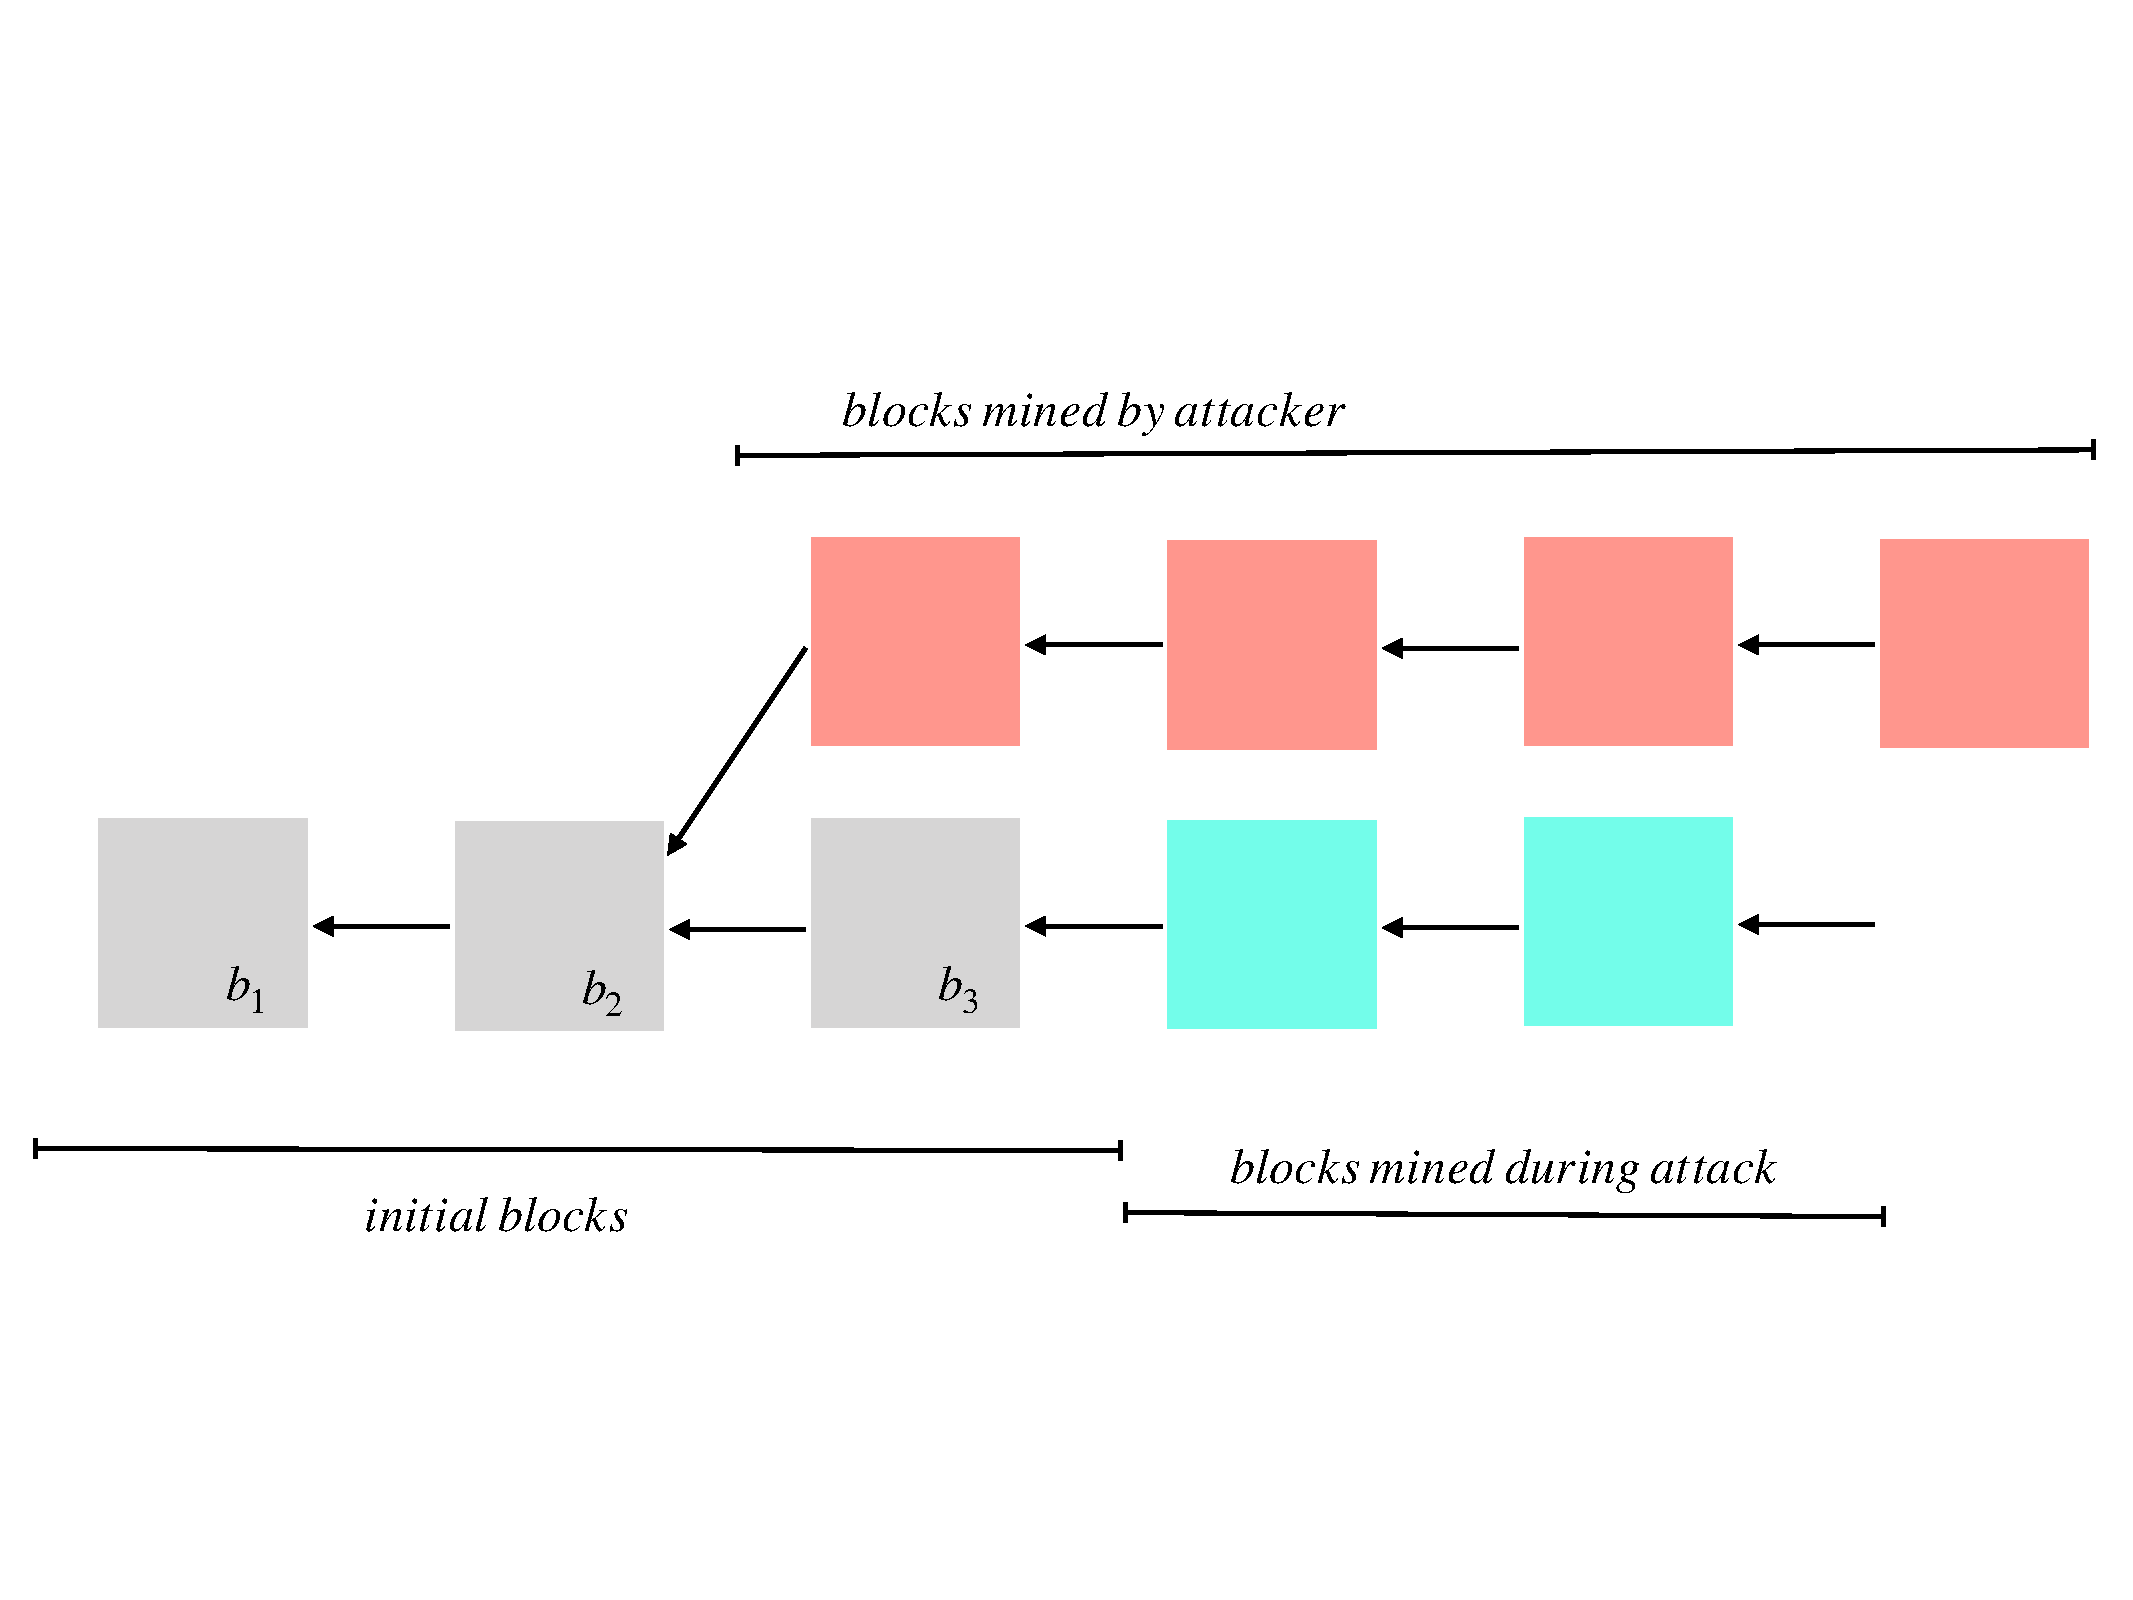
\includegraphics[width=\textwidth]{fig/51attack}
	\caption{A 51\% attack.}
	\label{fig:51}
\end{figure}

\subsection{Selfish mining}
In a selfish mining attack, the attacker does not violate the longest chain rule. Instead he violates the following mandate:
\begin{description}
	\item[Publication mandate] When a node finds a block, it should immediately announce this to the other processes. 
\end{description}
The idea behind not publishing the newest block is that it denies the other nodes to try and extend the longest chain. Thus, other nodes waist resources, trying to extend a chain, that is not the longest chain.

For a detailed description and analysis of selfish mining see 
 \href{https://disco.ethz.ch/courses/distsys/lnotes/chapter26.pdf}{Chapter 26.1} of these Lecture notes form ETH Zurich.

\begin{algorithm}
	\caption{Selfish mining}
	\begin{algorithmic}
		\State{\emph{Idea:} Mine secretly, without immediately publishing newly found blocks}
		\State{Let $l_p$ be length of the public chain}
		\State{Let $l_s$ be length of the secret chain}
		\If{a new block $b_p$ is published, i.e. $l_p$ has increased by 1}
			\If{$l_p>l_s$}
				\State{Start mining on $b_p$}
			\ElsIf{$l_p=l_s$}
				\State{Publish secretly mined block $b_s$}
				\State{Mine on $b_s$ and immediately publish new block}
			\ElsIf{$l_p=l_s-1$}
				\State{Push all secretly mined blocks}
			\EndIf
		\EndIf
	\end{algorithmic}
\end{algorithm}

\begin{note}
Results above show, that, if the attacker has more than $1/3$ of the hashing power, he can increase the ratio of blocks he creates in the blockchain by selfish mining.

\begin{itemize}
	\item If the attacker has more than $\alpha=1/3$ of the hashing power, he can increase the ratio of blocks he creates in the blockchain by selfish mining.
	\item If the attacker has more than $\alpha=1/4$ of the hashing power, and can reach $\gamma=0.5$ half of the nodes before another miner can reach them, he can benefit from selfish mining.
\end{itemize}
\end{note}

\section{P2P networking and network layer attacks}
A node in bitcoin does not maintain connections to all 10.000 bitcoin nodes.
Instead every node maintains a membership list, with addresses of other nodes. He maintains connections only to a few nodes selected at random from the list. 
We say that these connections form an overlay network.

In Bitcoin, nodes per default start by establishing 8 connections and extend this to up to 125 connections.

When a block is broadcast, every peer receiving the block first validates it and then forwards it to its neighbors. 

\subsection{Inventory messages and delivery denial attack}
The forwarding of a block consumes significant bandwidth. 
Bitcoin therefore uses \textsc{Inventory} messages to announce the a block to neighbors. Receiving an \textsc{Inventory} message a node would request to receive the actual message from only one of its neighbors. 

Nodes set a timeout when requesting a block. If they do not receive the block within the timeout, it is requested from a different source.

\begin{itemize}
	\item In bitcoin version 0.10, the timeout for receiving a block is set to 20 minutes.
\end{itemize}

\begin{definition}
In a \emph{delivery denial attack} a node does send \textsc{Inventory} messages, but when a block is requested, does not forward the block.	
\end{definition}

For extended details on this attack, see \href{https://scalingbitcoin.org/zh_HANS/papers/bitcoin-block-transaction-delivery.pdf}{[Gervais et. al. in CSS'15]}.
\question{What is the effect of this attack?}

\begin{note}
	Due to the static timeout, a delivery denial attack can significantly slow down block propagation.
	
	\begin{itemize}
		\item Slowing delivery of blocks increases the probability of a fork, as can be seen from Theorem~\ref{thm:fork}. This also increases the probability that a fork extends for several blocks.
		\item Slowing delivery of competing blocks may increase parameter $\gamma$ in the selfish mining scheme and thus make selfish mining more appealing and profitable even when $\alpha<1/4$.
	\end{itemize}
	
\end{note}

\subsection{Sybil attack}
In the eclipse attack, we assume that an attacker controls many IP addresses and machines, e.g. a botnet. 

\begin{definition}
	An attacker performing a \emph{sybil attack} registers multiple peers to receive as many connections as possible. Additionally, he may spread false network addresses. 
\end{definition}

\begin{note}
A successful attack has the following \textbf{effect:}
\begin{itemize}
	\item A successful attack allows the attacker to selectively reduce connectivity in the network. 
	\item If the attacker chooses to cooperate in the forwarding of a specific message, block or transaction, this may spread significantly faster. 
	\item Blocks or messages which the attacker chooses not to forward, may spread far slower.
	\item The increased network delay results in an increased fork probability.
	\item The selective connectivity gives the attacker an advantage, when performing selfish mining, i.e. increasing the $\gamma$ parameter.
\end{itemize}
\end{note}

\begin{idea} An interesting idea would be to select peers among the nodes that have previously published a block.
\end{idea}
\begin{note}
Using the idea above it is more difficult to introduce sybils. However, this would undo the anonymity of minors. Further, there is a bootstrapping problem.
\end{note}

\section{Attacks on transactions}
It is possible to issue two transactions that both spend the same outputs.
Only one of these transactions can be included in a chain, however, in case of a fork, each transaction may be included in a different branch of the fork.

Remember that a transaction counts as confirmed, if it is included in a block and a certain number of blocks is added on top of this block.

\begin{definition}
In a \emph{double spend attack} on an \emph{unconfirmed transaction} a payee accepts a transaction that is not confirmed, e.g. because he cannot wait for 20 minutes to sell a coffee. 

The payer then issues a different transaction an tries to get this different transaction included in the chain.
\end{definition}

\begin{definition}In a \emph{double spend attack} on a \emph{confirmed transaction} a payee accepts a confirmed transaction. 

The payer issues a different transaction an tries to get a fork including this transaction to become the longest chain.
\end{definition}

\begin{note}
We now look at the different attacks from Section~\ref{sec:attack}	and if they allow a double spend attack on confirmed transactions.
\begin{itemize}
	\item A 51\% attack allows to perform a successful double spend on a confirmed transaction. The attacker can simply create a secret fork including the second transaction, grow it to be longer than the public chain and publish once the original transaction is confirmed.
	\item During a selfish-mining attack it may happen that an attacker published a secret chain that is $l$ blocks or longer. Especially, if the attacker already has created a secret chain that is 6 blocks longer than the public chain, he is sure to succeed in a double spend attack.
	\item A sybil attack may increase the network latency and thus cause forks. However, the probability for a long fork is still quite small.
\end{itemize}
\end{note}

\begin{note}
	If attacker is doing selfish-mining, what is the probability that he currently is 6 blocks ahead (or more):
	\begin{itemize}
		\item If $\alpha=25\%$ then about 0.001.
		\item If $\alpha=33\%$ then about 0.01
	\end{itemize}
	These can be computed using the marginal probabilities from \href{https://disco.ethz.ch/courses/distsys/lnotes/chapter26.pdf}{Chapter 26.1} 
	
\end{note}


\subsection{Eclipse attack}
The eclipse attack is a special case of the sybil attack. It is performed similarly, but rather than targeting the complete network, the target is a individual node or small group of nodes.

\begin{definition}
	An attacker performing an \emph{eclipse attack} registers multiple peers to receive as many connections as possible. Additionally, he may spread false network addresses to the victims. 
	
The attacker aims to:
\begin{enumerate}[label=\Roman*]
	\item Monopolize all the connections of a single node or small part of the network.
\end{enumerate}
\end{definition}

\begin{note}
A successful attack has the following \textbf{effect:}
\begin{itemize}
	\item A successful attack may allow the attacker to exclude individual nodes from the network. The excluded nodes may no longer receive new blocks and any blocks created by the excluded nodes will probably be discarded when the attack stops.

This allows the attacker to double spend a confirmed transaction. By creating a chain especially for the attacked node, which confirms the transaction. The main chain will be longer and contain the other double spend transaction.
\end{itemize}	
\end{note}

\section{Updating a blockchain}
\label{sec:update}
Most blockchain protocols are under constant change. There are bugs and security vulnerabilities that are fixed and new features or improvement proposals added. 

As with other software, blockchain nodes do not accept and install updates instantly. For some controversial updates, notes might even choose to not update.

\comment{Since the initial version, published in 2009, Bitcoin has published about 50 versions. (Current 0.18.1)}

\begin{definition} An update that changes the rules, which blocks and transactions are valid, is called a \emph{fork}.
\end{definition}

\begin{note}
A software update that changes the code run by a node, but not its output is a \emph{non-fork}. Here nodes implementing new and old versions seamlessly work together.	
\end{note}

\subsection{Soft fork}
\begin{definition} A \emph{soft fork} is an update that makes some of the initial transactions or blocks, valid under a previous version invalid.
However all blocks and transactions under the new version are valid according to the old protocol.
\end{definition}

\begin{example}
A typical example of a soft fork is a security update, that rules out certain behaviors that were allows on the previous version.
\end{example}

\begin{note}
The result of a soft fork depends on whether a majority of the nodes switches to the new fork.
\begin{itemize}
	\item If the new version in a soft fork is accepted by less than 50\% of the nodes, these will create there own chain.
	\item If the new version in a soft fork is accepted by more than 50\% of the nodes, any block published on the old chain will eventually end in a short fork and be discarded.
\end{itemize}
\end{note}

\subsection{Hard fork}
\begin{definition} A \emph{hard fork} is an update that creates blocks that are not valid under the previous protocol.  
However blocks that are valid under the previous protocol are still valid under the new protocol.
\end{definition}

This version of a hard fork is also sometimes called a \emph{strictly extending hard fork}. It is generally considered easier to implement changes as a hard fork, than as a soft fork. 

\begin{example}
An example for a hard fork is a new feature introduced, e.g. a new Op code for scripts. Blocks and transactions that do not utilize this new feature are still valid under the new protocol.
\end{example}

\begin{note}
The result of a hard fork depends on whether a majority of the nodes switches to the new fork.
\begin{itemize}
	\item If the new version in a hard fork is accepted by less than 50\% of the nodes, any block published on the new chain will eventually end in a short fork and be discarded.
	\item If the new version in a hard fork is accepted by more than 50\% of the nodes, two chains will be created.
\end{itemize}
\end{note}

\subsection{Hard and soft forks}
\begin{definition} A \emph{hard and soft fork} is an update that creates blocks that are not valid under the previous protocol and also invalidates blocks from the previous protocol.
\end{definition}
This version of a hard fork is also sometimes called a \emph{bilateral hard fork}. 

\begin{note}
In a hard and soft fork, there will always be two chains created.
\end{note}

\question{Which fork are the following updates:
\begin{itemize}
	\item Increase maximum blocksize to 8MB.
	\item Decrease maximum blocksize to 0.5MB.
	\item Require blocksize of 5-6MB.
\end{itemize}}

\subsection{Analysis}
Forks that are caused by software or protocol updates have the potential to create forks of significant length. During such updates it may be easy to perform a double spending attack.

A safe variant is to require transactions to be included in both forks. However this is not possible for all variants, especially when spending outputs that where created in one of the forks.

There exist examples where a fork has resulted in two chains that where maintained separately.

\begin{idea} A common idea is for nodes to first signal their readyness to switch to a new version, e.g. in the blocks they publish.
This allows rules like:
\begin{itemize}
	\item Only move to the new version if 95\% of the last 2000 blocks have signaled to want to move to this version.
\end{itemize}
\end{idea}

\subsection{Pow as voting}
The discussion in Section~\ref{sec:update} shows that solving proof of work can be seen as majority voting, where every node has a voting share equivalent to the hashing power it is using to solve PoW. 

It is possible to take this view also for forks that occur during normal operation. A node votes by trying to find a block extending a certain chain.

Note especially that this voting mechanism has a build in sybil resistance, 
since voting requires limited resources, e.g. CPU or AISCS cycles and electricity. It is not possible to create a higher voting share, by simply creating new identities on the system.

